\appendix
\appendixpage

\begin{appendices}	
\chapter{Interview  Questionnaire}
This is considered as one of the best fact finding techniques. This includes direct interaction with the customer. It is considered as the best technique, because it is the only way the user can reveal the details and facts about his past, present and expected working, requirements, technologies, desertions to analysts. This is the information, which gives us the description of the system. we have to implement our logic and our own ideas and make this description to turn to a reality, to work as a real system which the user desires. 

In the following appendix, some example, structured interview and questionnaire sample documents are given. These documents have been used or can be used, directly or as a model, for gathering data under the context of this project.

\section{A List of Interview Questions Asked}
\subsection{List of Interview Questions Asked For the E-commerce}
\begin{itemize}
	\item What type of subscription fee do you prefer on  Guya E-commerce:-
	\begin{enumerate}
		\item Monthly Fixed Fee?
		\item Fee by Sells?
	\end{enumerate}
\end{itemize}

\subsection{List of Interview Questions Asked For the Express}
\begin{itemize}
	\item The first service (From Whom \& What), a sender receives; when he/she comes/arrives/inquires at the branch office.
	\item Summary of the whole management process; that takes place, in between a user and the service company.
	\item Questions From A Senders Point of View:-
	\begin{enumerate}
		\item How sender contact branch office and get info about destination?
		\item How track the courier and get update.
		\item How much is the cost to send a courier according to weight?
		\item What is the route of courier and estimated time needed to deliver the courier?
		\item How handle such acts like those that pending or return backed to the client etc.
		\item What happened if courier lost or damaged.
		\item Some other related services?
		\item How/Do provide delivery service for E-commerce.
	\end{enumerate}
	\item Questions From Express Services:-
	\begin{enumerate}
		\item Process of handling a customer (How and by whom), when he/she comes/arrives the first time.
		\item Booking process of a customer.
		\item The delivery process of a courier to a customer.
	\end{enumerate}
	\item Billing Process:-
	\begin{enumerate}
		\item How (and by whom) the bill payment process of a customer is done?
		\item What happen if the courier is redirected?
		\item Is there and advanced process related with the billing process?
	\end{enumerate}
\end{itemize}

\section{A Sample Questionnaire}
\subsection{A Sample Questionnaire For E-comnmerce}
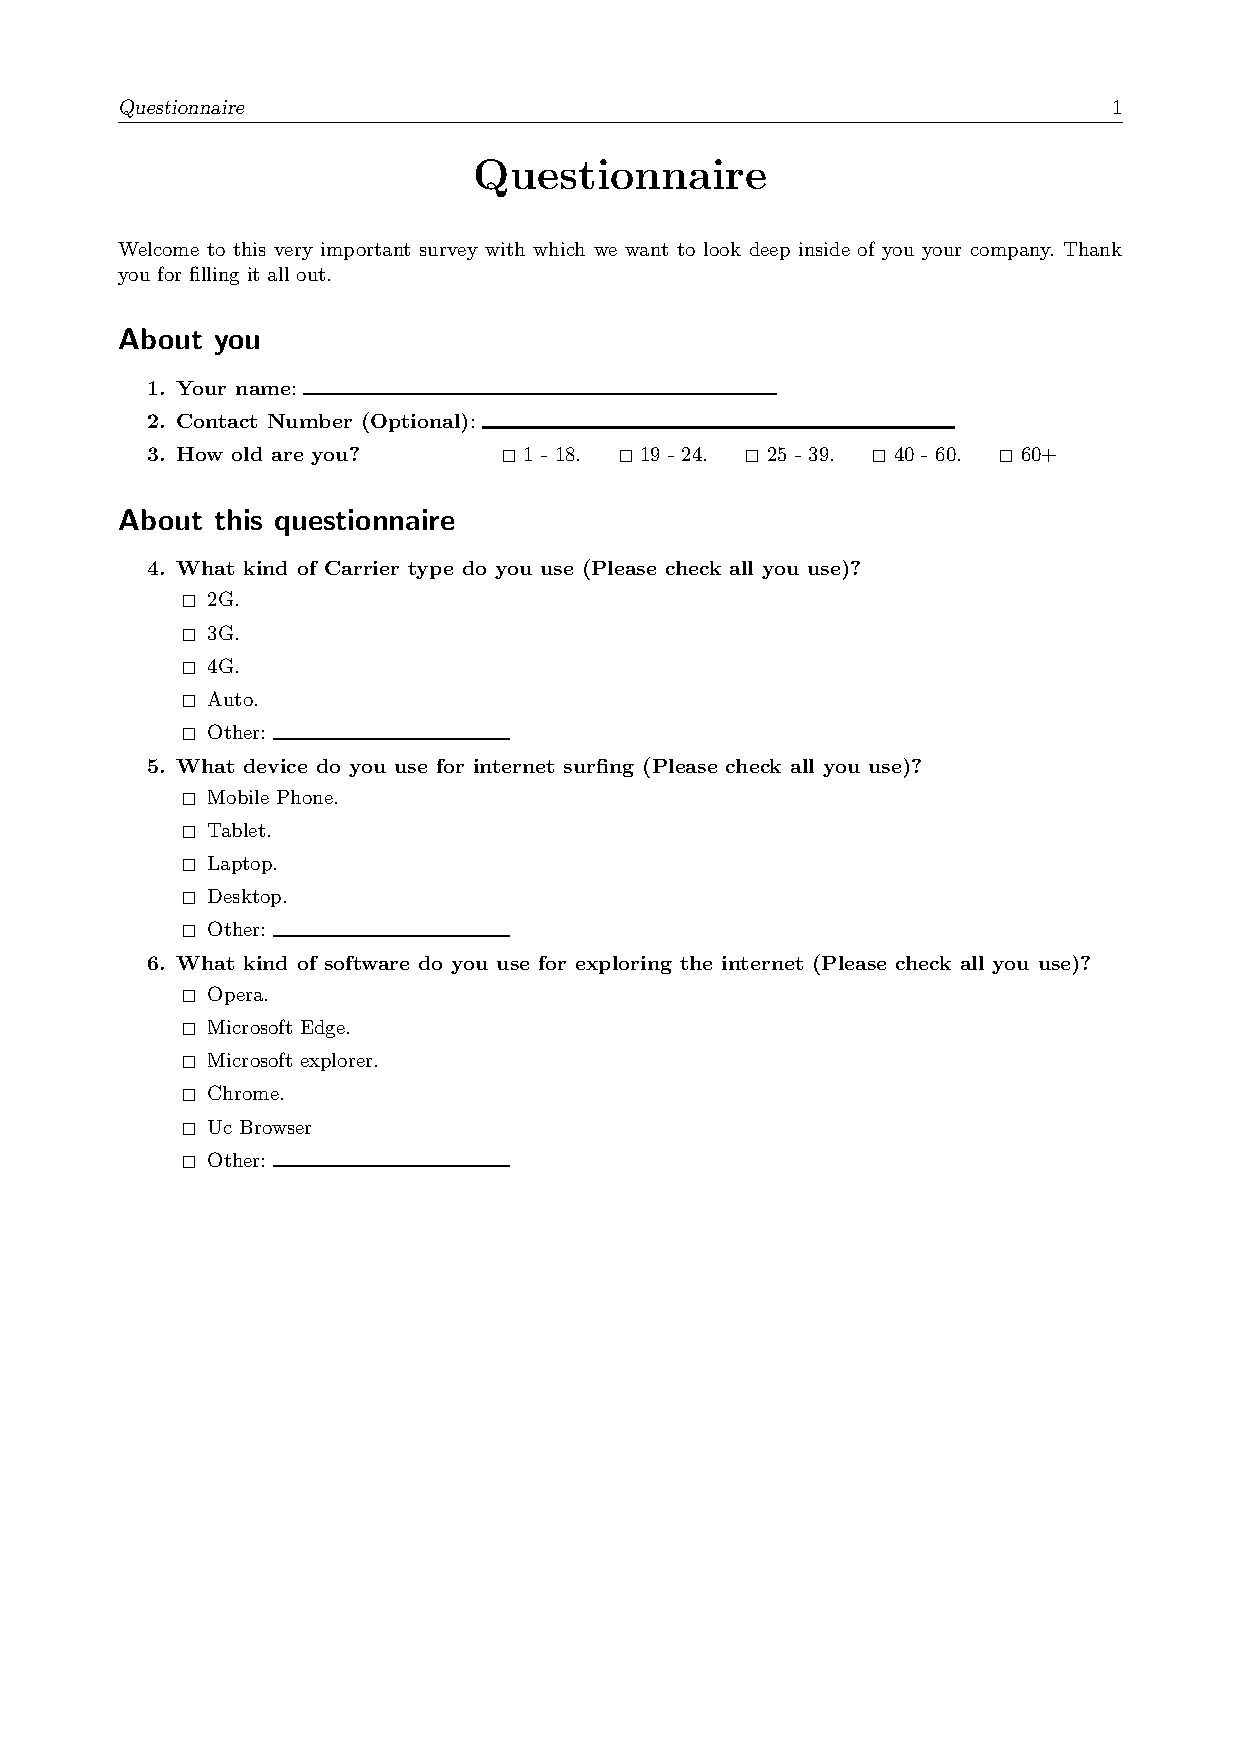
\includepdf{pdf/shop_questionnaire}
\subsection{A Smaple Questionnaire For Express}
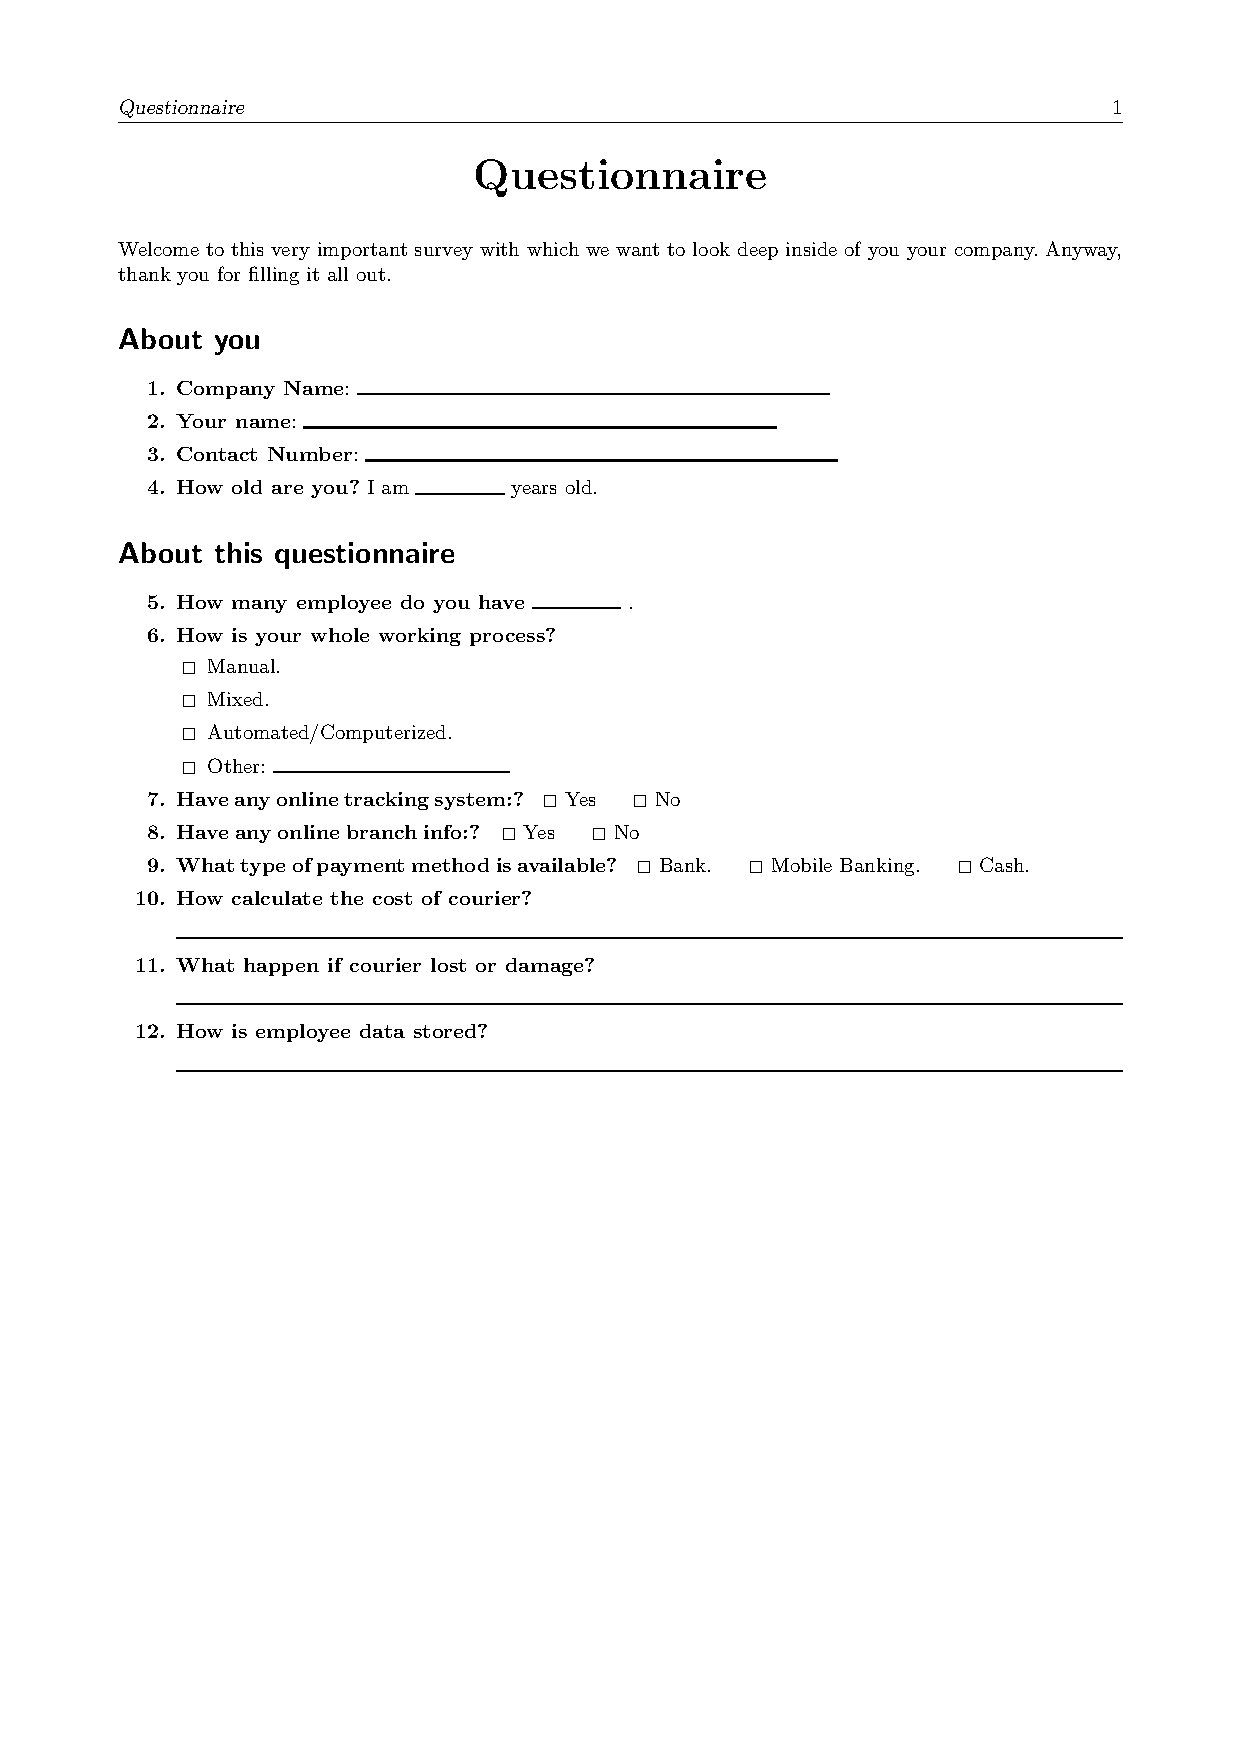
\includepdf{pdf/express_questionnaire}

%\chapter{Questionnaire Testing}
%\section{Appendix A. A List of Interview Questions Asked}
  
\chapter{Parcel Labeling Guide}
\subsection{Introduction}
\subsubsection{Purpose}
This section has been developed to make it easier to create and use labels on parcels shipped via the Guya Delivery System.

While some flexibility exists in design of shipping labels, using these standards will make label certification easier and make processing your parcels more efficient.

\subsubsection{Scope}
This section will focus primarily on the layout and content of domestic and ground shipping labels and will cover the following topics: 
\begin{itemize}
	% a, b, c
	\item Specifications for label elements
	\item Label examples displaying layout and content
	\item Applicable Intelligent Mail$^{TM}$ package barcode (IMpb) standards
\end{itemize}

\subsubsection{Audience}
This guideline is designed for use by any party interested in creating or understanding Guya parcel labeling requirements. This may include:
\begin{itemize}
	\item Third-party vendors developing shipping software applications
	\item Customers integrating Guya shipping capabilities in their custom shipping systems
	\item Integrators or Value Added Resellers (VARs) producing shipping labels
	\item Guya employees involved in label production, label processing, or assisting third-parties in label development
\end{itemize}


  
  
\chapter{Label Placement}
Improperly applied shipping labels can cause scanning problems and affect the quality of
tracking data provided by the Express. The following label placement guidelines will help ensure
maximum label scanning and processing.
\begin{itemize}
	\item Always place the label fully on the address side of the package without overlapping
the side or any other label.
	\item If for some reason, the Intelligent Mail package barcode appears on a separate label
from the delivery address, you should place the barcode above or to the left of the
delivery address with less than 1/2 inch between the label and the address.
	\item Do not cover the barcodes with tape or plastic wrap that may negatively impact
readability of these barcodes.
	\item When placing a barcode onto a convex or round object (such as a mailing tube), it is
very important that the barcode be placed on the package such that the bars of the
barcode are perpendicular to the curve of the item (note: if a parcel curves in more
than one direction, you should consider placing the item within a box or other flat-
sided container).
\end{itemize}
\begin{figure}[!h]
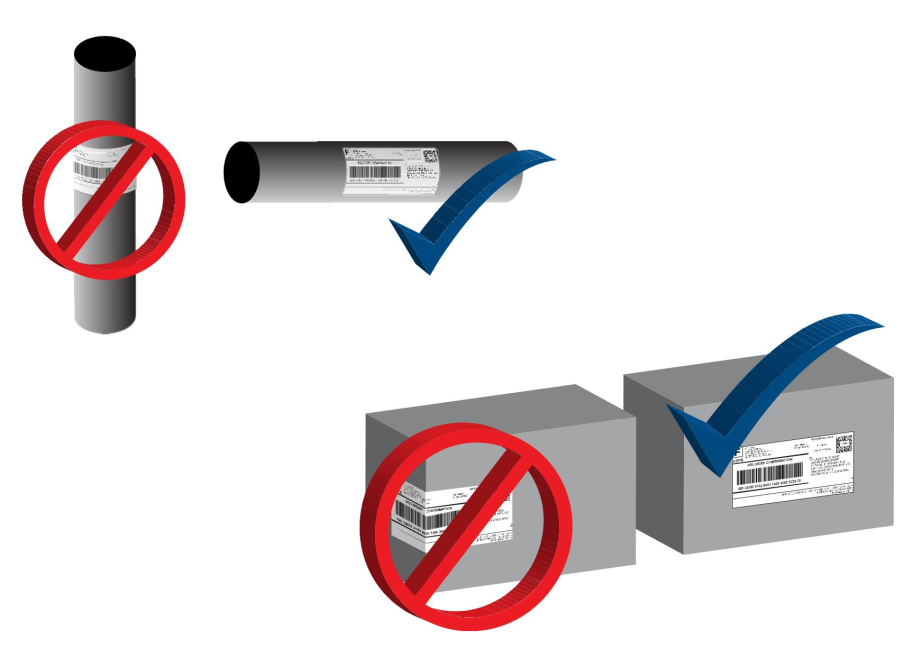
\includegraphics[width=15cm,keepaspectratio]{images/labeling_placement}
\caption{Label placement}
\end{figure}  
    
  
\chapter{Developer Manual}

\section{Live Demo}

\subsection{UI Framework Live Demo}
Visit a live demo of this template a http://bit.dev/guya-ltd/gcss

You can also consult the source code of this template at
http://github.com/Guya-LTD/bits
	
  
\section{Set It Up}

\begin{itemize}
	\item Install Docker(http://docker.io)
	\item Install Docker-compose(http://docker-compose.io)
	\item Clone\footnote{For more information see: https://help.github.com/articles/github-glossary\#clone} guya-ltd project from GitHub, or download it as a zip file
	\item Go to project root directory and
\end{itemize}


\section{Configure It}


  
\section{Deploy It}

\section{Develop It}

  
\chapter{Testing Information}
  
\section{Unit Testing Design}
List of scenarios to be tested for each user story.
 
\subsubsection{Browse Products}

\paragraph{List home products}
\begin{itemize}
	\item When the home page is requested, display all products of the shop.
	\item When no products found, show an informative message.
\end{itemize}

\paragraph{List products from a category}
\begin{itemize}
	\item When a category is requested, the chosen category will be indicated and its immediate children categories will be displayed, as well as all products belonging to that category or any descendant category.
	\item When the selected category does not exist, show a not found error message.
	\item When no products found, show an informative message.
\end{itemize}

\paragraph{Filter products by price}
\begin{itemize}
	\item When a price range filtering is requested in any product list page, the chosen price range will be displayed, as well as all products from the previous list (discarding any previous price filtering) whose price falls within the range.
	\item When minimum and maximum price are swapped, recover exchanging them.
	\item When invalid price provided, dismiss the price filter request.
	\item When no products found, show an informative message.
\end{itemize}

\paragraph{Filter products by color}
\begin{itemize}
	\item When a color filtering is requested in any product list page, the chosen color will be displayed, as well as all products from the previous list whose main color matches the selected color.
	\item When more than one color is selected at once, products whose main color matches any of the selected colors will be displayed.
	\item When no products found, show an informative message.
\end{itemize}

\paragraph{Show product detail}
\begin{itemize}
	\item When a product is requested, the chosen product will be displayed with all its information and pictures, as well as all the possible variants of that product.
	\item When the selected product does not exist, show a not found error message.
\end{itemize}

\paragraph{Show product variant detail}
\begin{itemize}
	\item When a product variant is requested, the chosen product variant will be displayed with all its information and pictures, as well as all other possible variants of that product.
	\item When the selected product variant does not exist, display the default variant instead.
	\item When the selected product does not exist, show a not found error message.
\end{itemize}
  
\subsubsection{Purchase Products}
\paragraph{Show cart detail}
\begin{itemize}
	\item When the shopping cart is requested, display the cart contents and the price details.
	\item When the shopping cart is empty, show an informative message.
\end{itemize}

\paragraph{Add item to cart}
\begin{itemize}
	\item When a product is requested to be added to the shopping cart, add the selected variant in the cart and display the updated cart content.
	\item When the product is already in the cart, the quantity will be updated with the addition.
	\item When the selected product does not exist, show a bad request error message.
\end{itemize}

\paragraph{Update item in cart}
\begin{itemize}
	\item When the quantity of an item in the shopping cart is requested to be updated in the cart detail page, replace the previous quantity with the new one provided and display the updated cart content.
	\item When the item does not exist in the cart, show a bad request error message.
	\item When the new quantity is invalid, show a bad request error message.
\end{itemize}

\paragraph{Remove item from cart}
\begin{itemize}
	\item When a product from the shopping cart is requested to be removed in the cart detail page, remove the item from the cart and display the updated cart content.
	\item When the item does not exist in the cart, show a bad request error message.
\end{itemize}

\paragraph{Start checkout}
\begin{itemize}
	\item When the checkout process is requested to start, display an order summary (i.e. cart content and price details) and the corresponding shipping and billing forms.
	\item When the shopping cart is empty, display the last visited page.
\end{itemize}

\paragraph{Finish checkout}
\begin{itemize}
	\item When the checkout process is requested to finish, display success message and all order details (i.e. cart content, price details, shipping and billing options).
	\item When invalid data provided, show a bad request error message and pre-fill the forms.
	\item When the shopping cart is empty, display the last visited page.
\end{itemize}
 
\subsubsection{User Management}
\paragraph{Show user profile}
\begin{itemize}
	\item When the user profile is requested, display the user data, change password and address book forms, as well as the list of orders from the user.
	\item When the user is not logged in, show an unauthorized error message and display login.
\end{itemize}

\paragraph{Do sign up}
\begin{itemize}
	\item When signing up a new user is requested, register the user and display the user profile.
	\item When user already registered, show a bad request error message and pre-fill form.
	\item When invalid data provided, show a bad request error message and pre-fill the form.
	\item 
\end{itemize}

\paragraph{Do log in}
\begin{itemize}
	\item When logging in a user is requested, sign in with the user and display the user profile.
	\item When invalid credentials provided, show an unauthorized error message and pre-fill form.
	\item When user already logged in, display the user profile.
\end{itemize}

\paragraph{Do log out}
\begin{itemize}
	\item When logging out a user is requested, sign out the user and display the last visited page.
	\item When user already logged out, display the last visited page.
\end{itemize}

\paragraph{Edit user data}
\begin{itemize}
	\item When the user data is requested to be updated, edit data and display updated user profile.
	\item When invalid data provided, show a bad request error message and pre-fill the form.
	\item When the user is not logged in, show an unauthorized error message and display login.
\end{itemize}

\paragraph{Edit user password}
\begin{itemize}
	\item When the user password is requested to be updated, change password and display user profile.
	\item When invalid current password provided, show a bad request error message.
	\item When the user is not logged in, show an unauthorized error message and display login.
\end{itemize}

\paragraph{Recover password}
\begin{itemize}
	\item When the user password is requested to be recovered, send email to the address provided with a temporary link to the recovery page, where the user can insert a new password.
	\item When the email provided does not exist, show a bad request error message and pre-fill form.
\end{itemize}

\paragraph{Add address to address book}
\begin{itemize}
	\item When an address is requested to be added to the address book in the user profile page, add
the selected address in the address book and display the updated user profile.
	\item When the address is invalid, show a bad request error message and pre-fill the form.
\end{itemize}

\paragraph{Update address in address book}
\begin{itemize}
	\item When an address is requested to be updated in the user profile page, replace the previous
address with the new provided and display the updated user profile.
	\item When the address does not exist in the address book, add it to the address book.
	\item When the address is invalid, show a bad request error message and pre-fill the form.
\end{itemize}

\paragraph{Remove address from address book}
\begin{itemize}
	\item When an address is requested to be removed in the user profile page, remove the address
from the address book and display the updated user profile.
	\item When the address does not exist in the address book, show a bad request error message.
\end{itemize}
 	
  
\subsection{Acceptance Tests Design}
Cucumber based list of rules.

\paragraph{Browse catalog}
\begin{itemize}
	\item Given I visit the web shop
	\item And I select a product
	\item When I add the product to the cart
  	\item And I go to the cart
	\item Then I have only the chosen item
	\item And the total price is correctly calculated
	\item When I add one more item
	\item Then the total price is correctly updated
\end{itemize}

\paragraph{Checkout}
\begin{itemize}
	\item Given I visit the web shop
	\item And I select a product
	\item When I add the product to the cart
	\item And I go to the checkout
	\item And I enter a valid address
	\item Then taxes are correctly calculated
	\item And the shipping methods are listed
	\item When I select a shipping method
	\item Then shipping cost is added to the total price
	\item And the payment form is displayed
	\item When I enter valid payment data
	\item And I finish the checkout
	\item Then I have purchased the product
\end{itemize}

\paragraph{Check order}
\begin{itemize}
	\item Given I visit the web shop	
	\item And I go to the signup page
	\item When I enter valid personal information
	\item Then I am successfully registered
	\item When I select a product
	\item And I add the product to the cart
	\item When I go to the checkout
	\item And I enter a valid address
	\item And I select a shipping method
	\item And I enter a valid payment data
	\item When I finish the checkout
	\item And I go to the user profile page
	\item And I go to the order history
	\item Then I have only one order
	\item When I select the order
	\item Then the total price is correct
	\item And the address is correct
	\item And the shipping method is correct
	\item And the payment is paid
\end{itemize}

\chapter{Ethiopia Post Code}
\section{Ethiopia Post Code Address Format}
\begin{figure}[!h]
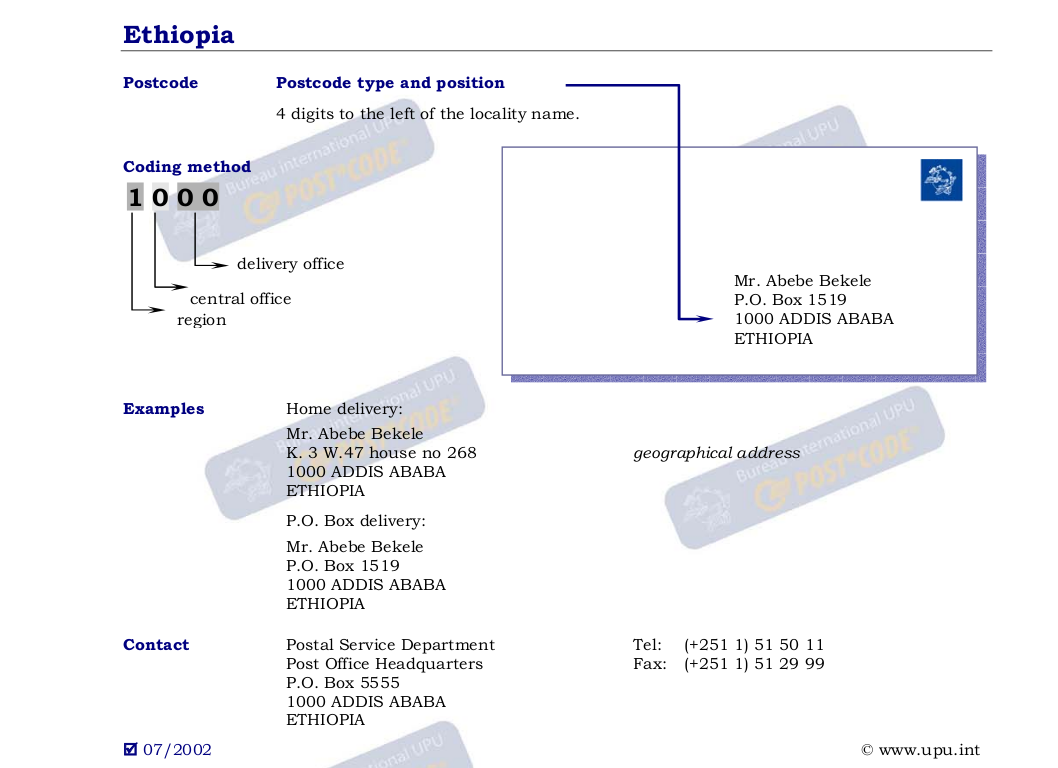
\includegraphics[width=15cm,keepaspectratio]{images/ethio_postcode_addressing}
\caption{Ethiopia Post Code Envelope and Address Format}
\end{figure}

\section{Ethiopia Postcodes Reference List}

\includepdf[page=-, pagecommand={}]{post-code-lists/post-codes.pdf}


\chapter{Azure Technologies}

\end{appendices}